% !TEX TS-program = lualatex
% !BIB TS-program = biber
%\documentclass[handout]{beamer}
\documentclass{beamer}
\newcommand{\misoclasstinytitleslide}{Partially based on material by:  Rob Fergus, Nikhil Srivastava,\\[-1em] 
Yiannis Koutis, Joshua Batson, Daniel Spielman}
%{Partially based on material by:  Branislav Kveton,  \\[-1em]  Partha Niyogi, Rob Fergus}
\newcommand{\misoclassdate}{}
\input{../common/misomva}\usetikzlibrary{arrows.meta}
\usepackage{verbatim}
\usepackage{listings}
\usepackage[customcolors]{hf-tikz}
\usepackage{color}
\usepackage{cancel}
%\usepackage[defaultmono]{droidmono}
\newcommand{\nbskip}{\vspace{-\baselineskip}}
%\newcommand{\hbskip}{\vspace{.5\baselineskip}}
\newcommand{\nhbskip}{\vspace{-.5\baselineskip}}

\definecolor{mygreen}{rgb}{0,0.6,0}
\definecolor{mygray}{rgb}{0.5,0.5,0.5}
\definecolor{mymauve}{rgb}{0.58,0,0.82}

\definecolor{Code}{rgb}{0,0,0}
\definecolor{Decorators}{rgb}{0.5,0.5,0.5}
\definecolor{Numbers}{rgb}{0.5,0,0}
\definecolor{MatchingBrackets}{rgb}{0.25,0.5,0.5}
\definecolor{Keywords}{rgb}{0,0,1}
\definecolor{self}{rgb}{0,0,0}
\definecolor{Strings}{rgb}{0,0.63,0}
\definecolor{Comments}{rgb}{0,0.63,1}
\definecolor{Backquotes}{rgb}{0,0,0}
\definecolor{Classname}{rgb}{0,0,0}
\definecolor{FunctionName}{rgb}{0,0,0}
\definecolor{Operators}{rgb}{0,0,0}
\definecolor{Background}{rgb}{0.98,0.98,0.98}

\lstset{ %
backgroundcolor=\color{white},   % choose the background color; you must add \usepackage{color} or \usepackage{xcolor}
basicstyle=\fdmfamily\footnotesize,        % the size of the fonts that are used for the code
breakatwhitespace=false,         % sets if automatic breaks should only happen at whitespace
breaklines=true,                 % sets automatic line breaking
captionpos=b,                    % sets the caption-position to bottom
commentstyle=\color{mygreen},    % comment style
deletekeywords={\dots},            % if you want to delete keywords from the given language
escapeinside={\%*}{*)},          % if you want to add LaTeX within your code
extendedchars=true,              % lets you use non-ASCII characters; for 8-bits encodings only, does not work with UTF-8
frame=single,	                   % adds a frame around the code
keepspaces=true,                 % keeps spaces in text, useful for keeping indentation of code (possibly needs columns=flexible)
language=Python,                 % the language of the code
% Comments
commentstyle=\color{Comments}\slshape,
% Strings
stringstyle=\color{Strings},
morecomment=[s][\color{Strings}]{"""}{"""},
morecomment=[s][\color{Strings}]{'''}{'''},
% keywords
morekeywords={import,from,class,def,for,while,if,is,in,elif,else,not,and,or,print,break,continue,return,True,False,None,access,as,,del,except,exec,finally,global,import,lambda,pass,print,raise,try,assert},
keywordstyle={\color{Keywords}\bfseries},
% additional keywords
morekeywords={[2]@invariant},
keywordstyle={[2]\color{Decorators}\slshape},
emph={self},
emphstyle={\color{self}\slshape},
otherkeywords={*,\dots},            % if you want to add more keywords to the set
numbers=left,                    % where to put the line-numbers; possible values are (none, left, right)
numbersep=5pt,                   % how far the line-numbers are from the code
numberstyle=\tiny\color{mygray}, % the style that is used for the line-numbers
rulecolor=\color{black},         % if not set, the frame-color may be changed on line-breaks within not-black text (e.g. comments (green here))
showspaces=false,                % show spaces everywhere adding particular underscores; it overrides 'showstringspaces'
showstringspaces=false,          % underline spaces within strings only
showtabs=false,                  % show tabs within strings adding particular underscores
stepnumber=1,                    % the step between two line-numbers. If it's 1, each line will be numbered
tabsize=2,	                   % sets default tabsize to 2 spaces
title=\lstname                   % show the filename of files included with \lstinputlisting; also try caption instead of title
}


\newcommand{\consindent}[1]{
    \begin{itemize}
        \item[{
\includegraphics[height=0.7\baselineskip]{../img/arrow_list}}] #1
    \end{itemize}
}


%%% part daniele
\usepackage{etex}
\TPshowboxesfalse
\textblockorigin{0mm}{0mm}

\definecolor{rouge1}{RGB}{226,0,38}  % red P
\definecolor{orange1}{RGB}{243,154,38}  % orange P
\definecolor{jaune}{RGB}{254,205,27}  % jaune P
\definecolor{blanc}{RGB}{255,255,255} % blanc P

\definecolor{rouge2}{RGB}{230,68,57}  % red S
\definecolor{orange2}{RGB}{236,117,40}  % orange S
\definecolor{taupe}{RGB}{134,113,127} % taupe S
\definecolor{gris}{RGB}{91,94,111} % gris S
\definecolor{bleu1}{RGB}{38,109,131} % bleu S
\definecolor{bleu2}{RGB}{28,50,114} % bleu S
\definecolor{vert1}{RGB}{133,146,66} % vert S
\definecolor{vert3}{RGB}{20,200,66} % vert S
\definecolor{vert2}{RGB}{157,193,7} % vert S
\definecolor{darkyellow}{RGB}{233,165,0}  % orange S
\definecolor{lightgray}{rgb}{0.9,0.9,0.9}
\definecolor{darkgray}{rgb}{0.6,0.6,0.6}

\setbeamertemplate{navigation symbols}{}
\setbeamertemplate{blocks}[rounded]
\setbeamercolor{block title}{bg=bleu2,fg=white}%bg=background, fg= foreground
\setbeamercolor{block body}{bg=lightgray}%bg=background, fg= foreground

\renewcommand{\sfdefault}{lmss}
\sffamily

%\newcommand{\ycol}[1]{\textcolor{darkyellow}{\textit{#1}}}

\newcommand{\rcolb}[1]{\textcolor{red}{\textit{\textbf{#1}}}}
\newcommand{\gcolb}[1]{\textcolor{vert3}{\textit{\textbf{#1}}}}
\newcommand{\bcolb}[1]{\textcolor{blue}{\textit{\textbf{#1}}}}
\newcommand{\ycolb}[1]{\textcolor{darkyellow}{\textit{\textbf{#1}}}}

\newcommand{\eqrcol}[1]{\textcolor{red}{#1}}
\newcommand{\eqgcol}[1]{\textcolor{vert3}{#1}}
\newcommand{\eqbcol}[1]{\textcolor{blue}{#1}}
\newcommand{\eqrcolb}[1]{\textcolor{red!70}{\mathbf{#1}}}
\newcommand{\eqgcolb}[1]{\textcolor{vert3!70}{\mathbf{#1}}}
\newcommand{\eqbcolb}[1]{\textcolor{blue!70}{\mathbf{#1}}}
\newcommand{\eqycol}[1]{\textcolor{darkyellow}{#1}}

%\newcommand{\otoprule}{\midrule[\heavyrulewidth]}

\colorlet{redp}{red!20} % vert S
\colorlet{greenp}{vert3!20} % vert S
\colorlet{bluep}{blue!20} % vert S

\usepackage{adjustbox}

\providecommand{\vareps}{\varepsilon}
% Highlight and cancel commands are defined in misomva.tex

\newcommand{\bookboxx}[1]{
\par\medskip\noindent
\framebox[\columnwidth]{
\begin{minipage}{0.98\columnwidth} {\par\smallskip#1\par\smallskip} \end{minipage} } \par\medskip }

\setbeamersize{text margin left=1cm,text margin right=1cm}
\tikzstyle{every picture}+=[remember picture]

\newcommand{\incarrow}{{
\includegraphics[height=0.7\baselineskip]{../img/arrow_list}}}
\newcommand{\consarrow}{{\hspace*{.1pt} 
\includegraphics[height=0.7\baselineskip]{../img/arrow_list}}\;}

% Change margins for slides
\newenvironment{changemargin}[2]{% 
  \begin{list}{}{% 
    \setlength{\topsep}{0pt}% 
    \setlength{\leftmargin}{#1}% 
    \setlength{\rightmargin}{#2}% 
    \setlength{\listparindent}{\parindent}% 
    \setlength{\itemindent}{\parindent}% 
    \setlength{\parsep}{\parskip}% 
  }% 
  \item[]}{\end{list}} 


\newcommand{\ie}{i.e.\xspace}
\newcommand{\eg}{e.g.\xspace}

\newcommand{\greycite}[1]{{\small \textcolor{gray}{\cite{#1}}}}
%%%

\begin{document}
% Topic-specific title slide

\newcommand{\topictitle}{Spectral Graph Sparsifiers: Theory}

\newcommand{\topicsubtitle}{Effective Resistance and Spielman-Teng Algorithm}
\renewcommand{\misoclasstinytitleslide}{Partially based on material by:  Rob Fergus, Nikhil Srivastava,\\[-1em] Yiannis Koutis, Joshua Batson, Daniel Spielman}

\MakeTopicSlide

\begin{frame}
\frametitle{Spectral Graph Sparsifiers}
Rayleigh-Ritz gives:
\pause 
\vspace{-0.5\baselineskip}
\[
\lambda_{\min} = \min \frac{\bx\transpose\bL\bx }{\bx\transpose\bx}
\quad \text{and} \quad 
\lambda_{\max} = \max \frac{\bx\transpose\bL\bx }{\bx\transpose\bx}
\]
\pause 
\questionbox{What can we say about $\lambda_i(G)$ and $\lambda_i(H)$?}
\pause 
\[
\alert{(1-\eps)} \bff\transpose\bL_{G}\bff  \leq  \bff\transpose\bL_{H}\bff  \leq  \alert{(1+\eps)} \bff\transpose\bL_{G}\bff 
\]
\pause 
\yellbox{Eigenvalues are approximated well!}
\[
\alert{(1-\eps)} \lambda_i(G)  \leq  \lambda_i(H)  \leq  \alert{(1+\eps)} \lambda_i(G) 
\]

\vspace{-0.5\baselineskip}
Using matrix ordering notation $(1-\varepsilon)\bL_{G} \preceq \bL_{H}  \preceq (1+\varepsilon) \bL_{G}$

\pause

\vspace{0.5\baselineskip}
\yellbox{As a consequence, $\argmin_{\bx} \norm{\bL_{H}\bx - \bb} \approx \argmin_{\bx} \norm{\bL_{G}\bx - \bb}$}
\end{frame}
\begin{frame}
    \frametitle{Spectral Graph Sparsifiers in ML}

%\bskip
\begin{proposition}[\small \cite{spielman2011graph, kyng2016framework}]
\normalfont
There exists an algorithm that can construct a spectral $\varepsilon$-sparsifier
\begin{itemize}%[leftmargin=*]
\pause
\item with only $\bigotime(n\log(n)/\varepsilon^2)$ edges
\pause
\item in $\bigotime(m\log^2(n))$ time and $\bigotime(n\log(n)/\varepsilon^2)$ space
\pause
\item a single pass over the data
\end{itemize}
\end{proposition}
\end{frame}
\begin{frame}
    \frametitle{Spectral Graph Sparsifiers in ML}
    %\frametitle{\large\textbf{\textcolor{bleu2}{\textsc{Graph Spectral Sparsification {in Machine Learning}}}}}
Laplacian smoothing (denoising): given $\:y \triangleq \:f^\star + \:\xi$ and $G$ compute\\
\begin{align}\label{eq:laprls}
%\argmin_{\:f \in \Re^n}  \tfrac{1}{n}\sum_{i=1}^n \left([\:y]_i - [\:f]_i\right)^2 + \gamma \sum_{e \in G} a_{e_{i,j}}([\:f]_i - [\:f]_j)^2\nonumber\\
\min_{\:f \in \Re^n}  %\tfrac{1}{n} 
(\:f - \:y)^\transp (\:f-\:y) + \lambda \:f^\transp \:L_G \:f
\end{align}

\pause
\begin{tabular}{@{}lccc}
& Preproc & Time & Space\\
$\wh{\:f} = (\lambda \:L_G + \:I)^{-1} \:y$ & $0$ & $\bigotime(m\log(n))$ & \hlr{$\bigotime(m)$}\\
\pause
$\wt{\:f} = (\lambda \:L_H + \:I)^{-1} \:y$ & \hlg{$\bigotime(m\log^2(n))$} & $\bigotime(n\log^2(n))$ & \hlg{$\bigotime(n\log(n))$}
\end{tabular}

\pause
\bskip
Large computational improvement\\
\consarrow accuracy guarantees! \greycite{sadhanala2016graph}

\pause
\hbskip
\begin{center}
\hfsetfillcolor{blue!10}
\hfsetbordercolor{blue}
%\tikzmarkin{regexists}(-9.6,0.5)(9.8,-0.25)
    \yellbox{Need to approximate spectrum only up to regularization level $\lambda$}
    %\tikzmarkend{regexists}
    \end{center}

\end{frame}
\begin{frame}
    \frametitle{\hlg{Ridge} Spectral Graph Sparsifiers in ML}
    %\frametitle{\large\textbf{\textcolor{bleu2}{\textsc{ Graph Spectral Sparsification}}}}
\begin{columns}
\column{\dimexpr\paperwidth-20pt}
\begin{definition}%[\small This paper]\label{def:eps-sparsifier}
	An \hlb{$(\vareps,\gamma)$-sparsifier} of $G$ is a reweighted subgraph $H$ s.t.
	%
	\hfsetfillcolor{vert3!10}
	\hfsetbordercolor{vert3}
	\begin{align}\label{eq:sparsif-quad-form}
	\tikzmarkin{epsgammaspars}(-7.9,0.4)(6.9,-0.25)
	(1-\vareps) \:L_G - \hleb{\varepsilon\gamma\bI} \preceq \:L_H \preceq (1 + \vareps) \:L_G + \hleb{\varepsilon\gamma\bI}
	\tikzmarkend{epsgammaspars}
	\end{align}
\end{definition}
\end{columns}

\pause
\bskip
Mixed \hlg{multiplicative}/\hlr{additive} error
\begin{itemize}
\item  large (\ie $\geq \gamma$) directions reconstructed accurately
\item  small (\ie $\leq \gamma$) directions uniformly approximated ($\gamma\bI$)
\end{itemize}
\pause
\hbskip
Adapted from Randomized Linear Algebra (RLA) community\\
\consarrow PSD matrix low-rank approx. \greycite{alaoui2014fast}
\pause
\hfsetfillcolor{vert3!10}
\hfsetbordercolor{vert3!80}
%\tikzmarkin{compimprov}(1.1,-0.2)(-0.2,0.)

\hbskip
RLA $\rightarrow$  Graph: Improve over $\cO(n\log n)$  exploiting regularization

Graph $\rightarrow$  RLA: Exploit $\laplacian_{G}$ structure for fast $(\varepsilon,\gamma)$-sparsification
%\tikzmarkend{compimprov}

\end{frame}
\begin{frame}
\frametitle{Spectral Graph Sparsification: Intuition}
%\frametitle{Spectral Graph Sparsifiers}
Let us consider unweighted graphs: $w_{ij} \in \{0,1\}$
\[
\bL_G = \sum_{ij} w_{ij}  \bL_{ij} = \sum_{ij\in E} \bL_{ij} \pause 
=  \sum_{ij \in E} (\bdelta_i - \bdelta_j)(\bdelta_i - \bdelta_j)\transpose \pause  = 
\sum_{e \in E} \bb_e\bb_e \transpose 
\]
\pause 
We look for a \emphcol{subgraph} $H$
\[
\bL_H = \sum_{e \in E} s_e \bb_e\bb_e \transpose 
\pause \quad \text{where $s_e$ is a new weight of edge e}
\]
\vspace{-1em}
\begin{center}
% TikZ replacement for sriva6 - Matrix sparsity pattern LG vs LH
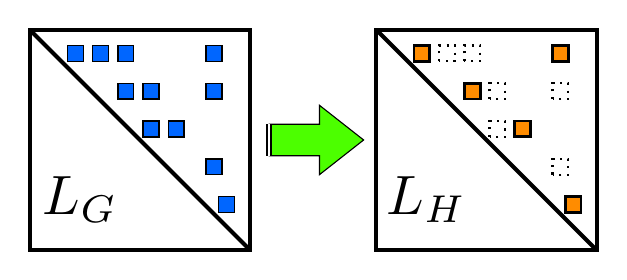
\begin{tikzpicture}[
    bsq/.style={fill=blue!60!cyan, draw=black, line width=0.5pt},
    osq/.style={fill=orange!90!yellow, draw=black, line width=1pt},
    dsq/.style={draw=black, dotted, line width=0.8pt},
    scale=0.8, transform shape
]
    \def\sz{3.5} \def\sq{0.25}
    % Left Matrix LG
    \draw[line width=1.5pt] (0,0) rectangle (\sz, \sz);
    \draw[line width=1.5pt] (0,\sz) -- (\sz, 0);
    \node at (0.8, 0.8) {\scalebox{2.5}{$L_G$}};
    \draw[bsq] (0.6, 3.0) rectangle ++(\sq, \sq); \draw[bsq] (1.0, 3.0) rectangle ++(\sq, \sq);
    \draw[bsq] (1.4, 3.0) rectangle ++(\sq, \sq); \draw[bsq] (2.8, 3.0) rectangle ++(\sq, \sq);
    \draw[bsq] (1.4, 2.4) rectangle ++(\sq, \sq); \draw[bsq] (1.8, 2.4) rectangle ++(\sq, \sq);
    \draw[bsq] (2.8, 2.4) rectangle ++(\sq, \sq); \draw[bsq] (1.8, 1.8) rectangle ++(\sq, \sq);
    \draw[bsq] (2.2, 1.8) rectangle ++(\sq, \sq); \draw[bsq] (2.8, 1.2) rectangle ++(\sq, \sq);
    \draw[bsq] (3.0, 0.6) rectangle ++(\sq, \sq);
    % Arrow
    \draw[fill=green!60!lime, draw=black] (3.8, 1.5) -- (4.6, 1.5) -- (4.6, 1.2) -- (5.3, 1.75) -- (4.6, 2.3) -- (4.6, 2.0) -- (3.8, 2.0) -- cycle;
    \draw[thick, double] (3.8, 1.5) -- (3.8, 2.0);
    % Right Matrix LH
    \begin{scope}[xshift=5.5cm]
        \draw[line width=1.5pt] (0,0) rectangle (\sz, \sz);
        \draw[line width=1.5pt] (0,\sz) -- (\sz, 0);
        \node at (0.8, 0.8) {\scalebox{2.5}{$L_H$}};
        \draw[osq] (0.6, 3.0) rectangle ++(\sq, \sq); \draw[dsq] (1.0, 3.0) rectangle ++(\sq, \sq);
        \draw[dsq] (1.4, 3.0) rectangle ++(\sq, \sq); \draw[osq] (2.8, 3.0) rectangle ++(\sq, \sq);
        \draw[osq] (1.4, 2.4) rectangle ++(\sq, \sq); \draw[dsq] (1.8, 2.4) rectangle ++(\sq, \sq);
        \draw[dsq] (2.8, 2.4) rectangle ++(\sq, \sq); \draw[dsq] (1.8, 1.8) rectangle ++(\sq, \sq);
        \draw[osq] (2.2, 1.8) rectangle ++(\sq, \sq); \draw[dsq] (2.8, 1.2) rectangle ++(\sq, \sq);
        \draw[osq] (3.0, 0.6) rectangle ++(\sq, \sq);
    \end{scope}
\end{tikzpicture}
\end{center}
\vspace{-1em}
\begin{flushright}
{\tiny \url{https://math.berkeley.edu/~nikhil/}}
\end{flushright}
\end{frame}
\begin{frame}
\frametitle{Spectral Graph Sparsification: Intuition}
%\frametitle{Spectral Graph Sparsifiers}
\[
\text{We want} \quad  (1-\varepsilon)\bL_{G} \preceq \bL_{H}  \preceq (1+\varepsilon)\bL_{G}
\]
\pause 
\[
\text{Equivalent, given\ } 
\bL_G = \sum_{e \in E} \bb_e\bb_e \transpose  \pause 
\text{\ find $\bs$, s.t.\ }   \bL_{G} \preceq \sum_{e \in E} s_e \bb_e\bb_e\transpose \preceq \kappa \cdot \bL_{G}
\]
\pause 
\[
\text{Forget $\bL$, given\ } 
\bA= \sum_{e \in E} \ba_e\ba_e \transpose  \pause 
\text{\ find $\bs$, s.t.\ }   \bA \preceq \sum_{e \in E} s_e \ba_e\ba_e\transpose \preceq \kappa \cdot \bA
\]
\pause 
\[
\text{Same as, given\ } 
\bI = \sum_{e \in E} \bv_e\bv_e \transpose  \pause 
\text{\ find $\bs$, s.t.\ }   \bI \preceq \sum_{e \in E} s_e \bv_e\bv_e\transpose \preceq \kappa \cdot \bI
\]
\pause 
\questionbox{How to get it?}
\pause 
$\bv_e \gets \bA^{-1/2}\ba_e$ \pause
\begin{center}
Then  $\sum_{e \in E} s_e\bv_e\bv_e \transpose \approx \bI \iff \sum_{e \in E} s_e\ba_e\ba_e\transpose \approx \bA$ \\
\notecol{\tiny\qquad multiplying by $\bA^{1/2}$ on both sides}
\end{center}

\end{frame}
\begin{frame}
\frametitle{Spectral Graph Sparsification: Intuition}
\bigskip
\questionbox{How does $\sum_{e \in E} \bv_e \bv_e\transpose = \bI$ look like geometrically?}
\pause 
\begin{center}
% TikZ replacement for sriva7 - Vectors in R^n
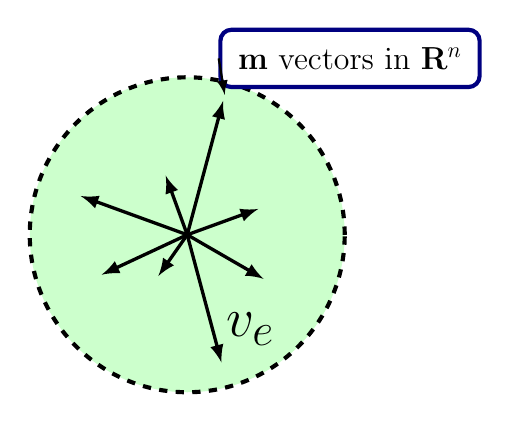
\begin{tikzpicture}[scale=0.8, transform shape]
    % Green circle with dashed border
    \filldraw[fill=green!20, draw=black, dashed, line width=1.5pt] (0,0) circle (2.5cm);
    % Vectors (arrows from center) with varying lengths
    \foreach \angle/\leqn in {20/1.2, 75/2.2, 110/1.0, 160/1.8, 205/1.5, 235/0.8, 285/2.1, 330/1.4} {
        \draw[->, >=latex, thick, line width=1.2pt] (0,0) -- (\angle:\leqn cm);
    }
    % Label ve
    \node at (1.0, -1.5) {\Huge $v_e$};
    % Text box
    \node[draw=blue!50!black, line width=1.5pt, rounded corners, fill=white, inner sep=8pt, anchor=west] (box) at (0.5, 2.8) {\Large \textbf{m} vectors in $\mathbf{R}^n$};
    % Arrow from box to a vector
    \draw[->, >=latex, thick] (box.west) -- (75:2.3cm);
\end{tikzpicture}
\end{center}
Decomposition of identity:  $\forall \bu$ (unit vector): $\sum_{e \in E} (\bu\transpose \bv_e)^2 = 1$ 
\pause 
\vspace{-0.5em}
\notecol{\tiny\qquad \qquad  moment ellipse is a sphere}
\vspace{-1em}
\begin{flushright}
{\tiny \url{https://math.berkeley.edu/~nikhil/}}
\end{flushright}
\end{frame}
\begin{frame}
\frametitle{Spectral Graph Sparsification: Intuition}
\bigskip
\questionbox{Example: What happens with $K_n$?}
\pause 
\begin{center}
$K_n$ graph \qquad  \qquad  \hfil $\sum_{e \in E} \bb_e \bb_e\transpose = \bL_G$ \hfil \qquad  \qquad  $\sum_{e \in E}  \bv_e \bv_e\transpose = \bI$ 
\resizebox{\columnwidth}{!}{%
\begin{tikzpicture}[
    node/.style={circle, fill=blue!70, draw=blue!90, minimum size=14pt, inner sep=0pt}
]

    % ===== Left: Complete graph K_6 =====
    \begin{scope}[xshift=0cm]
        % 6 nodes in hexagonal arrangement
        \foreach \i in {1,\dots,6} {
            \node[node] (n\i) at ({90 + (\i-1)*60}:1.8) {};
        }
        
        % All edges (complete graph)
        \foreach \i in {1,\dots,6} {
            \foreach \j in {\i,\dots,6} {
                \ifnum\i<\j
                    \draw[blue!80, thick] (n\i) -- (n\j);
                \fi
            }
        }
    \end{scope}
    
    % ===== Middle: Beige/peach circle with vectors =====
    \begin{scope}[xshift=6cm]
        % Beige filled circle with dashed boundary
        \fill[orange!15] (0,0) circle (2cm);
        \draw[dashed, very thick] (0,0) circle (2cm);
        
        % Vectors radiating (all same length)
        \foreach \angle in {0, 30, 60, 90, 120, 150, 180, 210, 240, 270, 300, 330} {
            \draw[-{Stealth[length=6pt]}, thick] (0,0) -- (\angle:1.5);
        }
    \end{scope}
    
    % ===== Right: Green ellipse with vectors =====
    \begin{scope}[xshift=12cm]
        % Green filled ellipse with dashed boundary
        \fill[green!20] (0,0) ellipse (2.2cm and 1.8cm);
        \draw[dashed, very thick] (0,0) ellipse (2.2cm and 1.8cm);
        
        % Vectors radiating (all same length)
        \foreach \angle in {0, 30, 60, 90, 120, 150, 180, 210, 240, 270, 300, 330} {
            \draw[-{Stealth[length=6pt]}, thick] (0,0) -- (\angle:1.4);
        }
    \end{scope}
    
\end{tikzpicture}
}
\end{center}
\pause 
\yellbox{It is already isotropic! (looks like a sphere)} \\
\pause 
\vspace{0.2em}
\notecol{\tiny\qquad rescaling $\bv_e = \bL^{-1/2}\bb_e$ does not change the shape }
\vspace{-1em}
\begin{flushright}
{\tiny \url{https://math.berkeley.edu/~nikhil/}}
\end{flushright}
\end{frame}
\begin{frame}
\frametitle{Spectral Graph Sparsification: Intuition}
\bigskip
\questionbox{Example: What happens with a dumbbell?}
\pause 
\begin{center}
Dumbbell \qquad  \qquad  \hfil $\sum_{e \in E} \bb_e \bb_e\transpose = \bL_G$ \hfil \qquad  \qquad  $\sum_{e \in E}  \bv_e \bv_e\transpose = \bI$ 
\resizebox{\columnwidth}{!}{%
\begin{tikzpicture}[
    node/.style={circle, fill=blue!70, draw=blue!90, minimum size=10pt, inner sep=0pt}
]

    % ===== Left: Dumbbell graph (two K6s connected) =====
    \begin{scope}[xshift=0cm]
        % Left clique K6 (6 nodes)
        \foreach \i in {1,\dots,6} {
            \node[node] (l\i) at ({90 + (\i-1)*60}:1.2) {};
        }
        % All edges in left clique
        \foreach \i in {1,\dots,6} {
            \foreach \j in {\i,\dots,6} {
                \ifnum\i<\j
                    \draw[blue!80, thick] (l\i) -- (l\j);
                \fi
            }
        }
        
        % Right clique K6 (6 nodes) - shifted right
        \begin{scope}[xshift=4.5cm]
            \foreach \i in {1,\dots,6} {
                \node[node] (r\i) at ({90 + (\i-1)*60}:1.2) {};
            }
            % All edges in right clique
            \foreach \i in {1,\dots,6} {
                \foreach \j in {\i,\dots,6} {
                    \ifnum\i<\j
                        \draw[blue!80, thick] (r\i) -- (r\j);
                    \fi
                }
            }
        \end{scope}
        
        % Bridge edge connecting the two cliques
        \draw[blue!80, thick] (l3) -- (r5);
    \end{scope}
    
    % ===== Middle: Beige vertical ellipse with clustered vectors =====
    \begin{scope}[xshift=9cm]
        % Beige filled vertical ellipse with dashed boundary
        \fill[orange!15] (0,0) ellipse (1.2cm and 2.2cm);
        \draw[dashed, very thick] (0,0) ellipse (1.2cm and 2.2cm);
        
        % Clustered vectors pointing upward (one group)
        \draw[-{Stealth[length=5pt]}, thick] (0,0) -- (80:1.5);
        \draw[-{Stealth[length=5pt]}, thick] (0,0) -- (90:1.6);
        \draw[-{Stealth[length=5pt]}, thick] (0,0) -- (100:1.4);
        \draw[-{Stealth[length=5pt]}, thick] (0,0) -- (70:1.3);
        \draw[-{Stealth[length=5pt]}, thick] (0,0) -- (110:1.3);
        
        % Clustered vectors pointing downward (another group)
        \draw[-{Stealth[length=5pt]}, thick] (0,0) -- (260:1.5);
        \draw[-{Stealth[length=5pt]}, thick] (0,0) -- (270:1.6);
        \draw[-{Stealth[length=5pt]}, thick] (0,0) -- (280:1.4);
        \draw[-{Stealth[length=5pt]}, thick] (0,0) -- (250:1.3);
        \draw[-{Stealth[length=5pt]}, thick] (0,0) -- (290:1.3);
        
        % Horizontal arrow touching ellipse edge
        \draw[-{Stealth[length=5pt]}, thick] (0,0) -- (0:1.2);
    \end{scope}
    
    % ===== Right: Green circle with clustered vectors + orange arrow =====
    \begin{scope}[xshift=14cm]
        % Green filled circle with dashed boundary
        \fill[green!20] (0,0) circle (2cm);
        \draw[dashed, very thick] (0,0) circle (2cm);
        
        % Clustered vectors pointing upward (one group)
        \draw[-{Stealth[length=5pt]}, thick] (0,0) -- (80:1.2);
        \draw[-{Stealth[length=5pt]}, thick] (0,0) -- (90:1.3);
        \draw[-{Stealth[length=5pt]}, thick] (0,0) -- (100:1.1);
        \draw[-{Stealth[length=5pt]}, thick] (0,0) -- (70:1.0);
        \draw[-{Stealth[length=5pt]}, thick] (0,0) -- (110:1.0);
        
        % Clustered vectors pointing downward (another group)
        \draw[-{Stealth[length=5pt]}, thick] (0,0) -- (260:1.2);
        \draw[-{Stealth[length=5pt]}, thick] (0,0) -- (270:1.3);
        \draw[-{Stealth[length=5pt]}, thick] (0,0) -- (280:1.1);
        \draw[-{Stealth[length=5pt]}, thick] (0,0) -- (250:1.0);
        \draw[-{Stealth[length=5pt]}, thick] (0,0) -- (290:1.0);
        
        % Orange arrow pointing right (the bridge edge) - touching circumference
        \draw[-{Stealth[length=8pt]}, orange, very thick] (0,0) -- (0:2);
    \end{scope}
    
\end{tikzpicture}
}
\end{center}
\pause 
\yellbox{The vector corresponding to the link gets stretched!} \\
\pause 
\vspace{0.2em}
\notecol{\tiny\qquad because this transformation makes all the directions important} \\
\pause 
\notecol{\tiny\qquad rescaling reveals the vectors that are critical}
\vspace{-1em}
\begin{flushright}
{\tiny \url{https://math.berkeley.edu/~nikhil/}}
\end{flushright}
\end{frame}


\begin{frame}[allowframebreaks]
\frametitle{References}
\printbibliography[heading=none]
\end{frame}

\MakeLastSlide
\end{document}
